\section{Pin Assignment}

During the compilation process described above, the Compiler was free to choose any
pins on the selected FPGA device to serve as inputs and outputs. However, an FPGA board
has hardwired connections between the pins of the FPGA chip and the other components that
are on the board.
We will use two toggle switches, labeled $SW_0$ and $SW_1$, to provide the
external inputs, $x_1$ and $x_2$, to our example circuit. These switches are connected
to the FPGA pins listed in Table \ref{tab:pinassign}. We will connect the output $f$ to a
light-emitting diode on your DE-series board. For the DE2-115 we will use a green LED: $LEDG_0$.
On the DE0-CV, DE1-SoC, DE10-Lite and DE10-Standard we will use $LEDR_0$. On the DE0-Nano and DE0-Nano-SoC, we will use $LED_0$
The FPGA pin assignment for the LEDs are listed in Table~\ref{tab:pinassign}.

\begin{table}[H]
\centering
\begin{tabular}{| c | c | c | c |}
\hline
Component & $SW_0$ & $SW_1$ & {\it LEDG}$_0$, {\it LED}$_0$, or {\it LEDR}$_0$ \\
\hline
DE0-CV & PIN$\_$U13 & PIN$\_$V13 & PIN$\_$AA2 \\
\hline
DE0-Nano & PIN$\_$M1 & PIN$\_$T8 & PIN$\_$A1 \\
\hline
DE0-Nano-SoC & PIN$\_$L10 & PIN$\_$L9 & PIN$\_$W15 \\
\hline
DE2-115 & PIN$\_$AB28 & PIN$\_$AC28 & PIN$\_$E21 \\
\hline
DE1-SoC & PIN$\_$AB12 & PIN$\_$AC12 & PIN$\_$V16 \\
\hline
DE10-Lite & PIN$\_$C10 & PIN$\_$C11 & PIN$\_$A8 \\
\hline
DE10-Standard & PIN$\_$AB30 & PIN$\_$AB28 & PIN$\_$AA24 \\
\hline
DE10-Nano & PIN$\_$Y24 & PIN$\_$W24 & PIN$\_$W15 \\
\hline
\end{tabular}
 
\caption{DE-Series Pin Assignments}
\label{tab:pinassign}
\end{table}

\begin{figure}[H]
   \begin{center}
      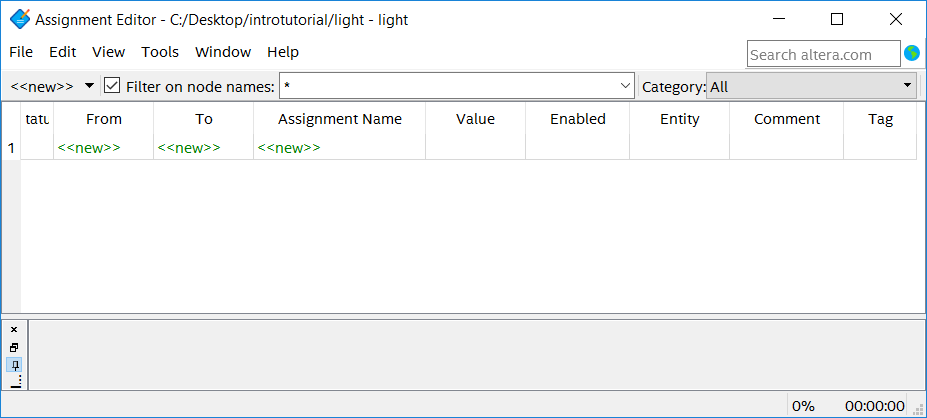
\includegraphics[scale=0.65]{figures/figure22.png}
   \caption{The Assignment Editor window.} 
	 \label{fig:22}
	 \end{center}
\end{figure}

Pin assignments can be made by using the {\it Assignment Editor}. 
Select {\sf Assignments $>$ Assignment Editor} to reach the window in Figure~\ref{fig:22}
(shown here as a detached window).
In the {\sf Category} drop-down menu select {\sf All}. Click on the {\sf $<$$<$new$>$$>$} button
located near the top left corner to make a new item appear in the table. Double-click the box
under the column labeled {\sf To} so that the {\sf Node Finder} button 

\includegraphics[scale=0.65]{figures/icon7.png}
appears. Click on the button (not the drop down arrow) to reach the window in 
Figure~\ref{fig:23}. Click on 
\includegraphics[scale=0.6]{figures/icon12.png} and 

\includegraphics[scale=0.6]{figures/icon15.png} to show or hide more search options.
In the {\sf Filter} drop-down menu select {\sf Pins: all}. Then, click the {\sf List} 
button to display the input and output pins to be assigned: $f$, $x1$, and $x2$.
Click on $x1$ as the first pin to be assigned and click the {\sf $>$} button; this action will 
enter $x1$ in the {\sf Nodes Found} box.  
Click {\sf OK}. The $x1$ node will now appear in the box 
under the column labeled {\sf To} in the Assignment Editor window. Alternatively, the node 
name can be entered directly by 
double-clicking the box under the {\sf To} column and typing in the node name.

Now double-click on the box to the right of this new $x1$ entry, in the column
labeled {\sf Assignment Name}, to open the drop-down menu in Figure~\ref{fig:24}. Scroll 
down and select {\sf Location (Accepts wildcards/groups)}. Instead of scrolling down the menu 
to find the desired item, you can alternatively type the first letter of the item in the 
{\sf Assignment Name} box. In this case the desired item happens to be the first item 
beginning with {\sf L}. Finally, double-click the box in the column labeled {\sf Value}.
Type the pin assignment corresponding to $SW_0$ for your DE-series board, as listed in 
Table \ref{tab:pinassign}.

Use the same procedure to assign input $x2$ and output $f$ to the appropriate pins listed in
Table \ref{tab:pinassign}. An example using a DE1-SoC board is shown in Figure~\ref{fig:25}.
To save the assignments made, choose {\sf File $>$ Save}. You can also simply close 
the Assignment Editor window, in which case a pop-up box will ask if you want to save
the changes to assignments; click {\sf Yes}. Finally, execute the {\sf Processing $>$ 
Start Compilation} command to create a new circuit that makes use of your pin assignments. 

\begin{figure}[H]
   \begin{center}
      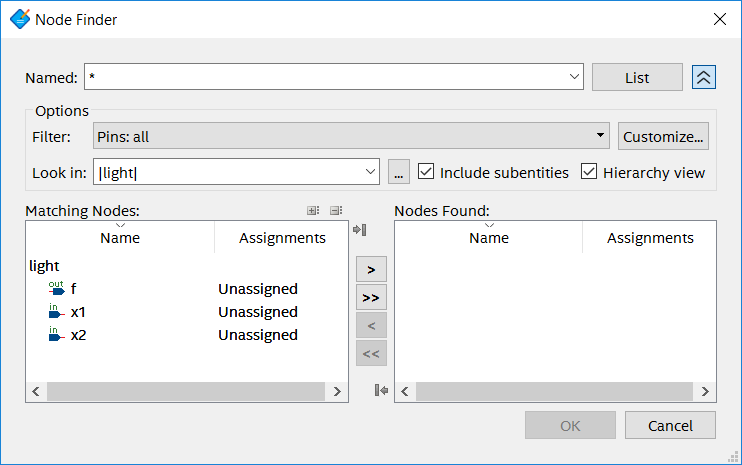
\includegraphics[scale=0.65]{figures/figure23.png}
   \caption{The Node Finder displays the input and output names.} 
	 \label{fig:23}
	 \end{center}
\end{figure}

\begin{figure}[H]
   \begin{center}
      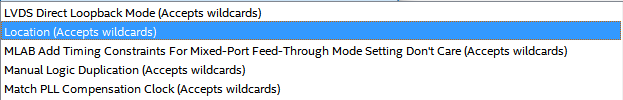
\includegraphics[scale=0.75]{figures/figure24.png}
   \caption{The available assignment names for a DE-series board.} 
	 \label{fig:24}
	 \end{center}
\end{figure}

\begin{figure}[H]
   \begin{center}
      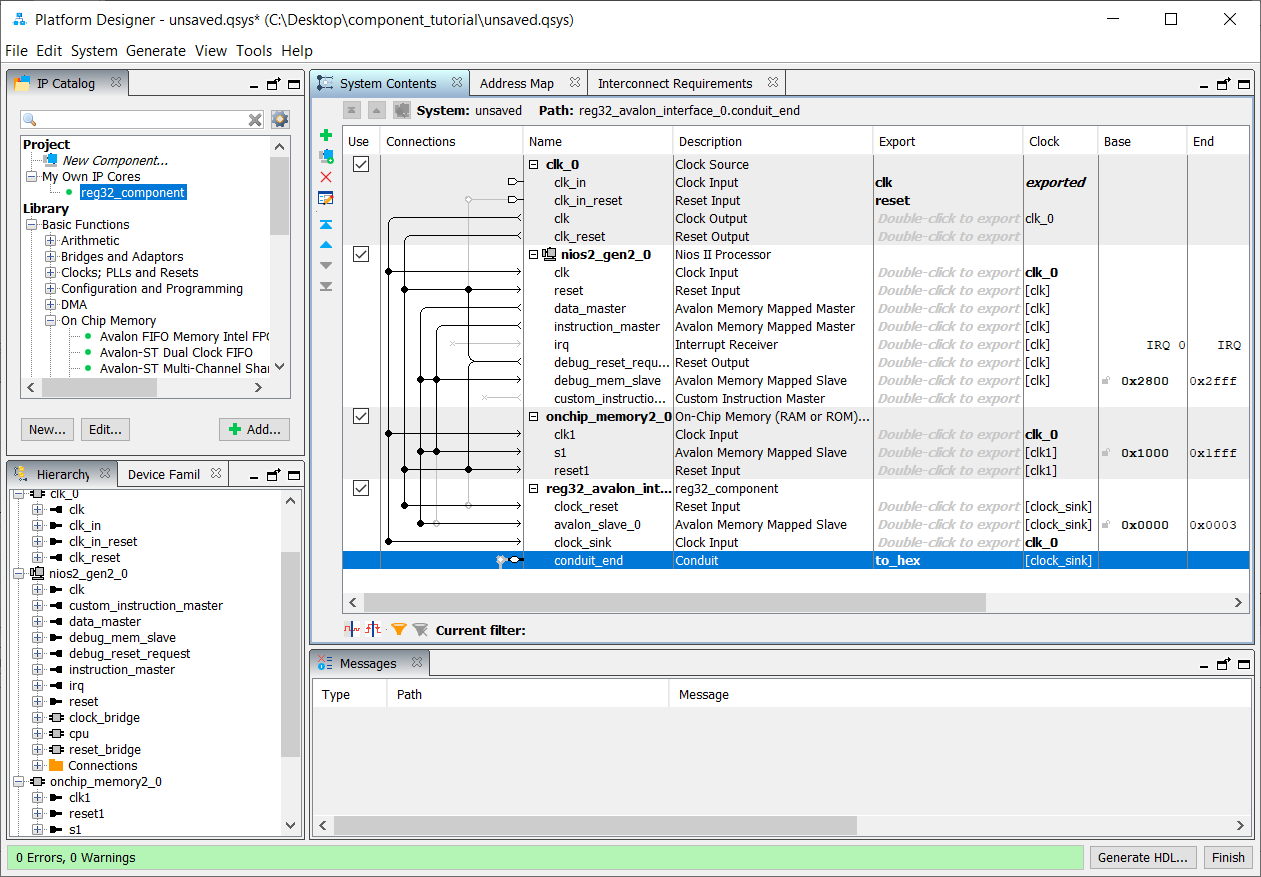
\includegraphics[scale=0.65]{figures/figure25.png}
   \caption{The complete assignment.} 
	 \label{fig:25}
	 \end{center}
\end{figure}

When you make assignments related to your project, such as the pin assignments described
above, or the device assignments made earlier in the tutorial, Quartus Prime stores these 
assignments in a special type of file associated with your project. This file is called 
a {\it quartus settings file} ({\it qsf}), and in our case would be named {\it light.qsf}. 
In this file the pin assignments created above (using a DE1-SoC board as an example) would
be included as

\begin{center}
\begin{verbatim}
	set_location_assignment PIN_AB12 -to x1
	set_location_assignment PIN_AC12 -to x2
	set_location_assignment PIN_V16 -to f
\end{verbatim}
\end{center}

A useful Quartus Prime feature allows the user to import into a project the assignments
contained in a quartus settings file, rather than creating them manually using the 
Assignment Editor.  Importing pin assignments from an existing {\it qsf} file can be a
convenient way of making these assignments, rather than following the (somewhat tedious)
process described above.   

\noindent
You can import pin assignments by choosing {\sf Assignments $>$ Import Assignments}. 
This command opens the dialogue in Figure~\ref{fig:27}, allowing you to select a file to import. 
 
\begin{figure}[H]
   \begin{center}
      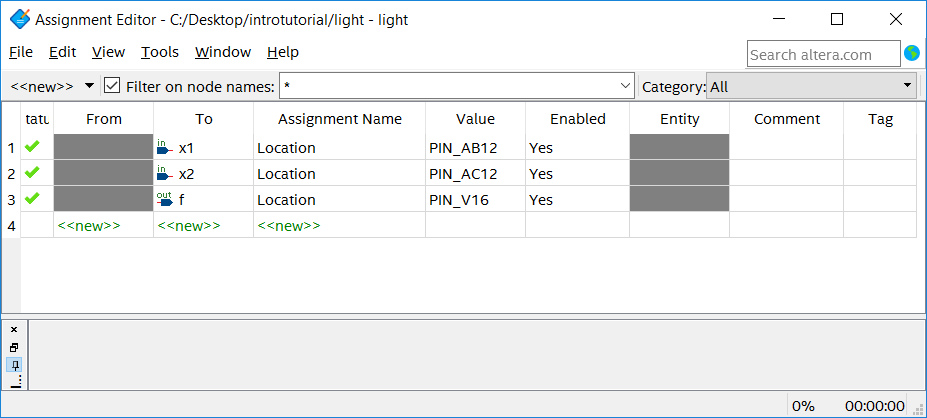
\includegraphics[scale=0.65]{figures/figure27.png}
   \caption{Importing the pin assignment.} 
	 \label{fig:27}
	 \end{center}
\end{figure}
